\chapter{Análise e Design}

%Neste capitulo temos como objetivo analisar e detalhar a solução  de acordo com os requisitos pedidos pela empresa  levantados no capitulo 3.Por isso devemos ter uma visão geral da arquitetura e modelagem que devera ser utilizada, através dos diagramas.
Neste capítulo temos como objetivo analisar e detalhar a solução de acordo com os requisitos pedidos pela empresa, levantados no capítulo 3. Para isso será necessária uma visão geral da arquitetura e modelagem que deverá ser utilizada, através dos diagramas
\newpage
\section{Fluxograma}

A melhor definição de fluxograma é “um mapa gráfico rico em informações que descreve claramente as etapas do processo, suas tomadas de decisão, fornecendo documentação onde for necessário”.\cite{Gradus2019} 

Além da descrição citada, é importante observar que há muitas razões para se usar o fluxograma, por exemplo:
\begin{itemize}
	\item Melhorar o entendimento do processo através do apelo visual;
	\item Diagnosticar onde se necessita melhorias;
	\item Mostrar a sequência em que as etapas são executadas, permitindo identificar ações que possam ser eliminadas;
	\item Identificar melhorias que podem ser feitas imediatamente;
	\item Descreve qualquer tipo de processo, dos simples aos complexos;
	%\item
	\item Detalha o funcionamento de todas as partes do processo;
	\item Fácil uso
	\item Fácil interpretação
\end{itemize}
\newpage


\begin{figure}[H]
	\caption{\label{fluxograma2teste}Fluxograma da\textit{ Smart Solution}}%
	\begin{center}
		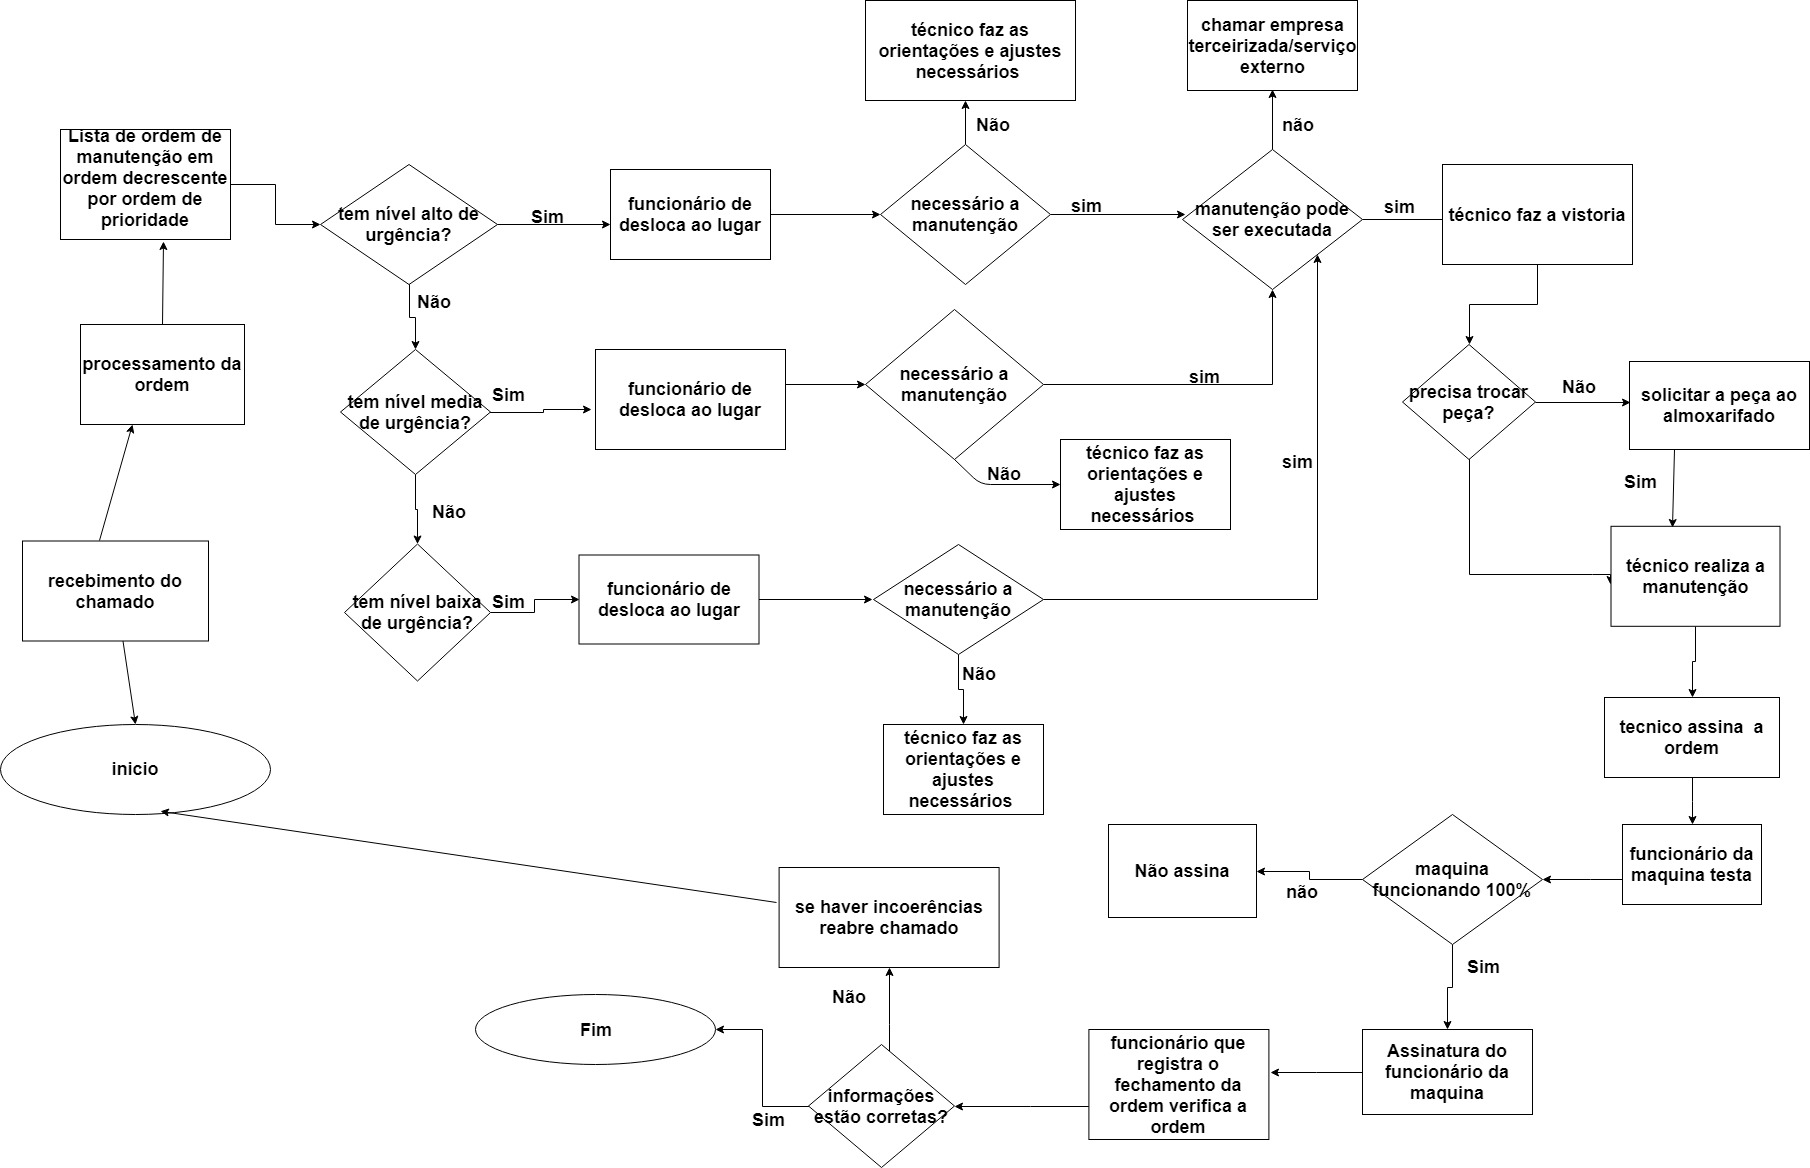
\includegraphics[scale=0.40,angle=90]{Figuras/fluxograma2teste}
		
	\end{center}
	%	\legend{Fluxograma do Sistema}
\end{figure}
\newpage
%descrever fluxograma
O fluxograma começa recebendo a ordem de serviço do SAP e vai para o processamento para colocar em sua lista de prioridades designada  , após isso é verificado se precisa que o técnico se desloque até a máquina ou apenas orientar o usuário os procedimentos a adotar, mas se for necessário técnico faz a vistoria e verifica de precisara de peça ou não , após isso o funcionário da máquina faz a vistoria  em seguida e coletado as assinaturas e se estiver tudo certo fecha a ordem de serviço.

\newpage

\section{Diagrama de Caso de Uso}
% ---

O diagrama de casos de uso é o diagrama mais geral e informal da UML, utilizado normalmente nas fases de levantamento e análise de requisitos do sistema,
embora venha a ser consultado durante todo o processo de modelagem e possa
servir de base para outros diagramas. Apresenta uma linguagem simples e de
fácil compreensão para que os usuários possam ter uma ideia geral de como o
sistema irá se comportar. Procura identificar os atores (usuários, outros sistemas ou até mesmo algum hardware especial) que utilizarão de alguma forma 
o software, bem como os serviços, ou seja, as funcionalidades que o sistema
disponibilizará aos atores, conhecidas nesse diagrama como casos de uso.\cite{guedes2009uml}


\begin{figure}[H]
	\caption{\label{novocasodeusointegra}Diagrama de Caso de Uso Desenvolvido para o projeto Smart Solution}
	\begin{center}
		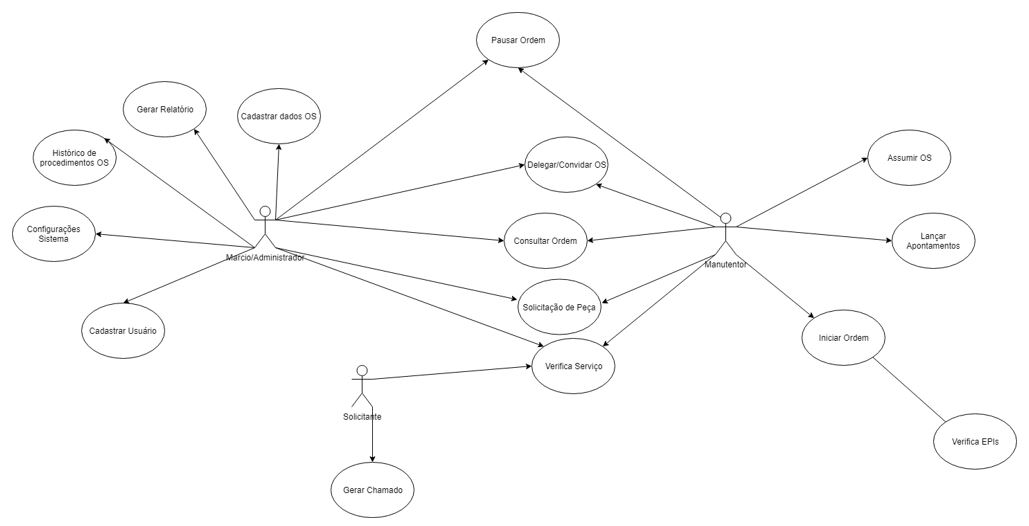
\includegraphics[scale=0.90,angle=90]{./Figuras/novocasodeusointegra}
		
	\end{center}
	%	\legend{Diagrama de Caso de Uso}
\end{figure}

\newpage
%descriçao caso de uso
O caso de uso possui como atores administrador geral de TI, márcio, responsável pela máquina e manutentor. O administrador tem visão geral de todas as informações provenientes das ordens de serviços como de seus procedimentos, históricos disponíveis. O márcio faz a atribuição das ordens de serviço assim como a impressão e pós realização confere a ordem de serviço para assim assinar e retornar ao SAP as informações contidas na ordem de serviço. O responsável da máquina e responsável por uma das assinaturas mediante uma vistoria de sua máquina de uso. O manutentor realiza a manutenção e solicita peças ao almoxarifado se for necessário a troca de alguma peça.



\section{Diagrama de Classes}
%---
O diagrama de classes é provavelmente o mais utilizado e é um dos mais importantes da UML. Serve de apoio para a maioria dos demais diagramas. Como o
próprio nome diz, define a estrutura das classes utilizadas pelo sistema, determinando os atributos e métodos que cada classe tem, além de estabelecer como
as classes se relacionam e trocam informações entre si.\cite{guedes2009uml}

\newpage
\begin{figure}[H]
	\caption{\label{Diagrama_de_classe_integrado}Diagrama de classe para \textit{Smart Solution}}
	\begin{center}
		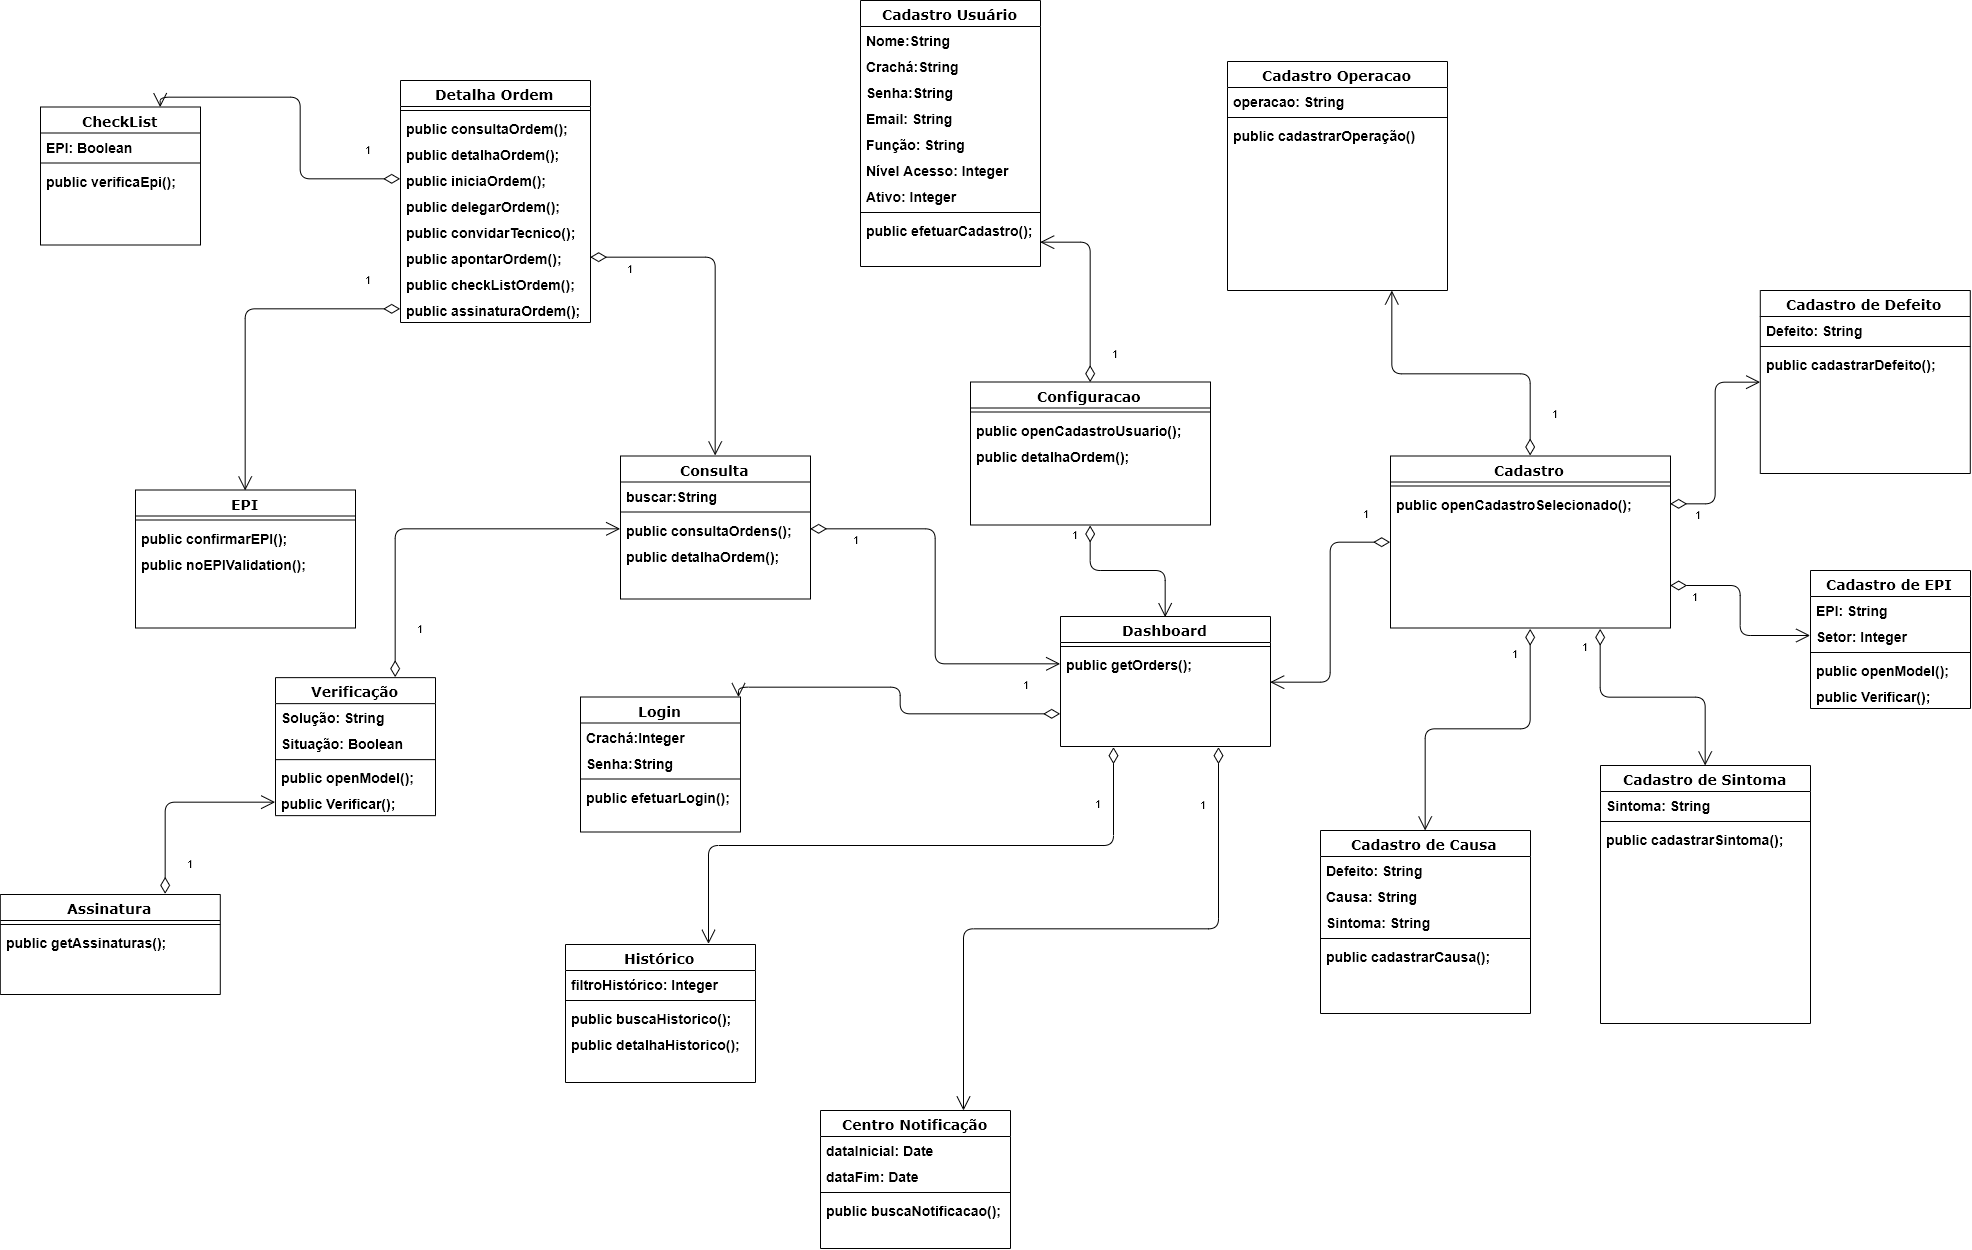
\includegraphics[scale=0.35, angle=90]{./Figuras/Diagrama_de_classe_integrado}
		
	\end{center}
	%	\legend{Diagrama de Classe}
\end{figure}

\newpage

Neste diagrama está a base das classes do projeto\textit{ Smart Solution} , visando ter telas com suas regras de negócio variáveis que o sistema deveria ter, além de começarmos a modelar possíveis dados recebidos. Dentro desta base temos uma classe de login para usuário efetuar o mesmo, banco de dados para armazenamento das ordens de manutenção , assinaturas para finalidade de pegar as assinaturas de cada responsável pelo processo , outras telas como setor solicitante, equipamento que está com problemas e solicitar peças do estoque ,dados da manutenção que e recebido via SAP.

\newpage
\section{Diagrama de Atividades}


O diagrama de atividade
preocupa-se em descrever os passos a serem percorridos para a conclusão de uma
atividade específica, podendo esta ser representada por um método com certo
grau de complexidade, um algoritmo, ou mesmo por um processo completo. O
diagrama de atividade concentra-se na representação do fluxo de controle de
uma atividade.\cite{guedes2009uml}



\begin{figure}[H]
	\caption{\label{diagramaDeAtividades}Diagrama de Atividades no desenvolvimento do software \textit{Smart Solution}}
	\begin{center}
		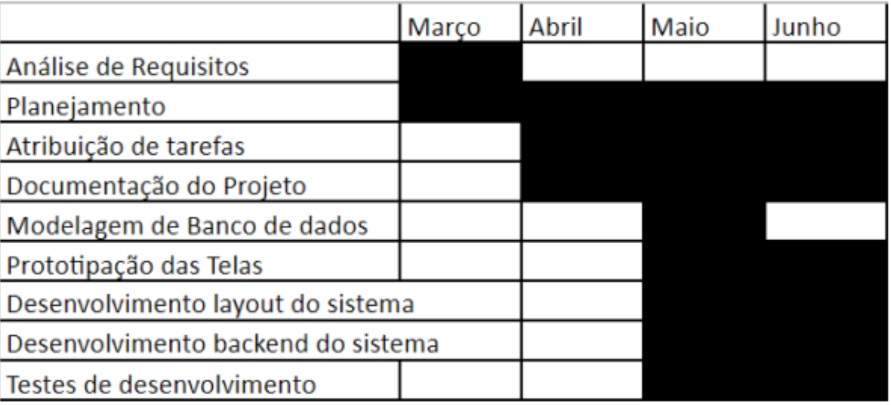
\includegraphics[scale=0.72 ]{./Figuras/diagramaDeAtividades}
		
	\end{center}
	%	\legend{Diagrama de Atividades}
\end{figure}
%\section{Diagrama de Sequencia}
%\section{Modelo de Dados}
%\subsection{Modelo Lógico da Base de Dados}
%\subsection{Criação física do Modelo de Dados}
%\subsection{Dicionário de Dados}
\newpage
\section{Ambiente de Desenvolvimento}


%36Capítulo 4.  Análise e DesignÉ uma plataforma utilizada para o desenvolvimento de aplicações Web.-Node Js: Interpretador de código javascript. -Ionic: Utilizado para o de-senvolvimento de aplicativos móveis híbridos. Git: Sistema de controle deversões distríbuido, é utilizado para o versionamento de código.
%Foi utilizado minha maquina que possui SSD 240 gb processador i3 com 4 gigas de RAM , mause teclado configuração semelhante dos meus companheiros.
%Também foi utilizado para desenvolver o software , a sala de aula, em casa, grupo de whatsapp e gitHub para todos terem a ultima versão.

As linguagens utilizadas serão as seguintes: Javascript - Uma linguagem de alto nível, dinâmica e fracamente tipada, muito utilizada atualmente; TypeScript - Um superconjunto de Javascript que traz várias adições a linguagem, foi desenvolvido pela Microsoft; Tecnologias Utilizadas - MySQL: Utilizada para o gerenciamento de dados; Angular: É uma plataforma utilizada para o desenvolvimento de aplicações Web; Node.Js: Interpretador de código javascript; Ionic: Utilizado para o desenvolvimento de aplicativos móveis híbridos; Git: Sistema de controle de versões distribuído, é utilizado para o versionamento de código. Para que houvesse o desenvolvimento mútuo do projeto se fez necessário um ambiente adequado com as ferramentas necessárias, das quais o SENAI foi responsável por fornece-las.
\newpage

\section{Sistemas e Componentes Externos Utilizados}

%GitHub: Plataforma de hospedagem de código fonte, nela serão armazenados os códigos do projeto, facilitando o acesso a diferentes versões de desenvolvimento aos desenvolvedores.
GitHub do Smart Solution \footnote{\url{https://github.com/senai-duasrodas}}: Plataforma de hospedagem de código fonte, nela serão armazenados os códigos do projeto, facilitando o acesso a diferentes versões de desenvolvimento aos desenvolvedores, possibilitando o desenvolvimento em conjunto de toda a equipe.

\newpage

